%%%%%%%%%%%%%%%%%%%%%%%%%%%%%%%%%%%%%%%%%
% University/School Laboratory Report
% LaTeX Template
% Version 3.1 (25/3/14)
%
% This template has been downloaded from:
% http://www.LaTeXTemplates.com
%
% Original author:
% Linux and Unix Users Group at Virginia Tech Wiki 
% (https://vtluug.org/wiki/Example_LaTeX_chem_lab_report)
%
% License:
% CC BY-NC-SA 3.0 (http://creativecommons.org/licenses/by-nc-sa/3.0/)
%
%%%%%%%%%%%%%%%%%%%%%%%%%%%%%%%%%%%%%%%%%

%----------------------------------------------------------------------------------------
%	PACKAGES AND DOCUMENT CONFIGURATIONS
%----------------------------------------------------------------------------------------

\documentclass{ctexart}

\usepackage[version=3]{mhchem} % Package for chemical equation typesetting
\usepackage{siunitx} % Provides the \SI{}{} and \si{} command for typesetting SI units
\usepackage{graphicx} % Required for the inclusion of images
\usepackage{natbib} % Required to change bibliography style to APA
\usepackage{amsmath} % Required for some math elements 
%\usepackage{showframe} % for showing page frames


\setlength\parindent{0pt} % Removes all indentation from paragraphs

\renewcommand{\labelenumi}{\alph{enumi}.} % Make numbering in the enumerate environment by letter rather than number (e.g. section 6)

%\usepackage{times} % Uncomment to use the Times New Roman font

%==========pesusdo codes
\usepackage[linesnumbered,boxed]{algorithm2e}
%\renewcommand{\algorithmcfname}{算法}
\renewcommand{\repeat}{Repeat}

%==========citation===========
%\usepackage{cite}
\usepackage{url}


% ==========添加首行缩进,两个字符===========
\usepackage{indentfirst}
\setlength{\parindent}{2em}
% ==========强制图片位置===========
\usepackage{float}

% ==========特殊数学符号===========
\usepackage{mathtools}
\usepackage{dsfont}
\usepackage{amsfonts}
% ==========列表===========
\usepackage{enumerate}

%----------------------------------------------------------------------------------------
%	DOCUMENT INFORMATION
%----------------------------------------------------------------------------------------

\title{模型调优——基本概念,调参方法等} % Title

%\author{fengmi \textsc{Feng}} % Author name

\author{Mia Feng} % Author name

\date{\today} % Date for the report

\begin{document}

\maketitle % Insert the title, author and date

%\begin{center}
%\begin{tabular}{l r}
%Date Performed: & January 1, 2012 \\ % Date the experiment was performed
%Partners: & James Smith \\ % Partner names
%& Mary Smith \\
%Instructor: & Professor Smith % Instructor/supervisor
%\end{tabular}
%\end{center}

% If you wish to include an abstract, uncomment the lines below
% \begin{abstract}
% Abstract text
% \end{abstract}

%----------------------------------------------------------------------------------------
%	SECTION 1
%----------------------------------------------------------------------------------------

\section{概述}
模型过拟合时,有高方差,可能是因为使用了相关数据中过多的参数;模型欠拟合时,有高偏差,意味着模型过于简单,无法发现训练数据集中隐含的模式,这会使得模型应用于未知数据时性能不佳。

当在不同的训练数据集上多次重建模型时,偏差可以从总体上衡量预测值和实际值的差异,此时的偏差衡量的是系统误差。但是当在同一训练集的不同子集上训练是,方差用来衡量模型对特定样本示例预测的一致性(或者说变化)。可以说模型对训练数据中的随机性是敏感的。基于此,有两种方法进行模型选择(fine tuning)。一种是holdout,将数据分为训练集,验证集和测试集。根据在验证集上的预测评分来调优拟合训练集的参数,最终在测试集上预测。但是缺点是模型对训练数据的随机性敏感。相比之下,k折交叉验证评价的鲁棒性更好。通过将数据不放回抽样分为k个子集,每次选取其中的k-1个子集组成训练集拟合,另外的一个子集作为验证集评分,总共迭代k次。最后以k次评分的均值作为模型的平均性能估计。注意k值过大会使得评价方差过高。当数据中类别比例相差较大时,推荐分层交叉验证,sklearn中为StratifiedKFold

Bias-variance tradeoff 是通过引入正则化调整模型的复杂度。正则化可以有效的解决特征间高度相关的问题。增加正则化的强度会导致权重系数逐渐收缩。

如何判断是高偏差还是高方差,以及根据此选择参数,见下图


\begin{figure}[H]
\begin{center}
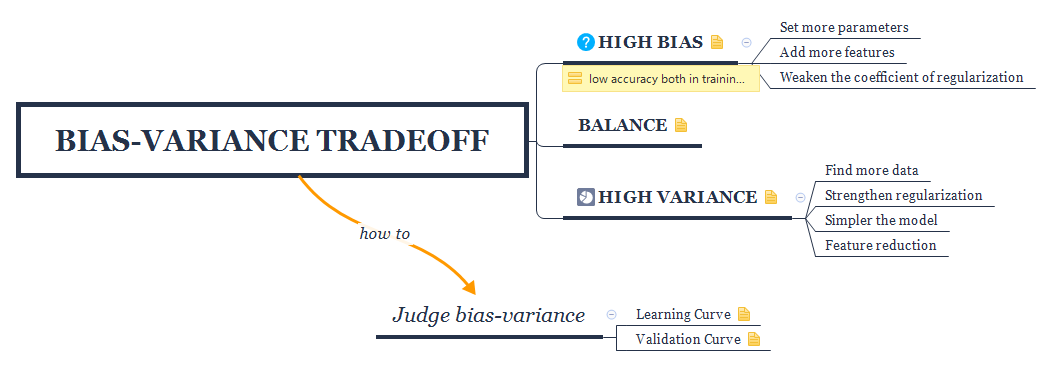
\includegraphics[width=1\textwidth]{fig/Bias-variance tradeoff.png} % Include the image placeholder.png
\caption{模型调优策略}
\end{center}
\end{figure}


%To determine the atomic weight of magnesium via its reaction with oxygen and to study the stoichiometry of the reaction (as defined in \ref{definitions}):

求解目标:分类超平面,以二维空间为例,求解一条直线
\begin{equation}
y = b+\theta_1x_1+\theta_2x_2=\theta^{\mathbf{T}}x+b
\end{equation}

求解思路:最小化误分类点数(由其可以扩展到SVM最大化最小几何距离)。Concretely, 通过最小化代价函数\cite{LiHang:Statistic}:
\begin{equation}
L\big(\theta,b \big)=-\sum\limits_{x_i\in M}y_i\big(\theta\cdot x_i+b\big)
\end{equation}

求解方法:最小化误分类点数,stochastic gradient descent

\subsection{推导}
\label{derivations}
\begin{description}
\item[误分类点数]
当分类结果正确时,类标乘以分类平面$\big(\theta\cdot x_i+b\big)$所得符号为正,反之所得符号为负。所以,对类标乘以分类平面值的结果取负,记为误分类的点数目。目标要对其求极小
\begin{equation}
\arg\min\limits_{\theta,b}L\big(\theta,b \big)=-\arg\min\limits_{\theta,b}\sum\limits_{x_i\in M}y_i\big(\theta\cdot x_i+b\big)
\end{equation}

\item[Stochastic gradient descent]
每次随机选取一个误分类点使其梯度下降,因为对所有样本点的梯度下降是耗时的(这种叫做Batch Gradient Descent)。神经网络采用SGD与Batch Gradient Desecent的中间版,或者这种中间版的改进版。为了降低运算量,采用mini-batch gradient descent(对数据分批次求极小)。算法在期望上收敛,所以不一定是全局最优。即使代价函数是强凸且光滑,收敛速度也只有$O\left(\frac{1}{T}\right)$,where $T$是样本点数。运用随机梯度下降后,每当一个实例点被误分,即位于超平面错误的一侧时,即调整$\theta,b$使得分类平面向该误分类点的一侧移动,以减少该误分类点与超平面的距离,甚至超平面越过该误分类点使其被正确分类\cite{LiHang:Statistic}。
\begin{equation}
\begin{array}{lcl}
\nabla_{\theta}L\big(\theta,b\big)=-\sum\limits_{x_i\in M}y_ix_i \\
\nabla_{b}L\big(\theta,b\big)=-\sum\limits_{x_i\in M}y_i
\end{array}
\end{equation}
\end{description}

%
%\begin{equation}
%\begin{align*}
%&\max\limits_{w,b}\quad \gamma\\
%& \begin{array}{r@{\quad}r@{}l@{\quad}l}
%s.t.&\sum\limits_{j=1}^m a_{ij} x_j&\leq b_i,  &i=1,2,3\ldots,n\\
% &x_j&\geq110,  &i=1,2,3\ldots,n  \\
% &x_j&\geq10,  &i=1,2,3\ldots,n  \\
% &x_j&\geq0,  &i=1,2,3\ldots,n  \\
%& x_j&\geq0,  &i=1,2,3\ldots,n  \\
%\end{array} .
%\end{align*}


%----------------------------------------------------------------------------------------
%	SECTION 2
%----------------------------------------------------------------------------------------

\section{算法实现}
见\cite{LiHang:Statistic}
%
\begin{enumerate}[1.]
\item 初始化$\theta,b$
\item 迭代直至训练集中无误分类点\{
\begin{enumerate}[a.]
\item 从样本集中随机选取数据点$\big(x_i,y_i\big)$
\item 如果 $y_i\big(\theta\cdot x_i+b\big)\leq0$
\begin{equation}
\begin{array}{lcl}
\theta \leftarrow \theta+\eta y_ix_i\\
b\leftarrow b+ \eta y_i
\end{array}
\end{equation}
\end{enumerate}
\}
\end{enumerate}

%----------------------------------------------------------------------------------------
%	SECTION 3
%----------------------------------------------------------------------------------------
%
\section{Implementation}
分类测试:数据在flowers.csv
\begin{figure}[H]
\begin{center}
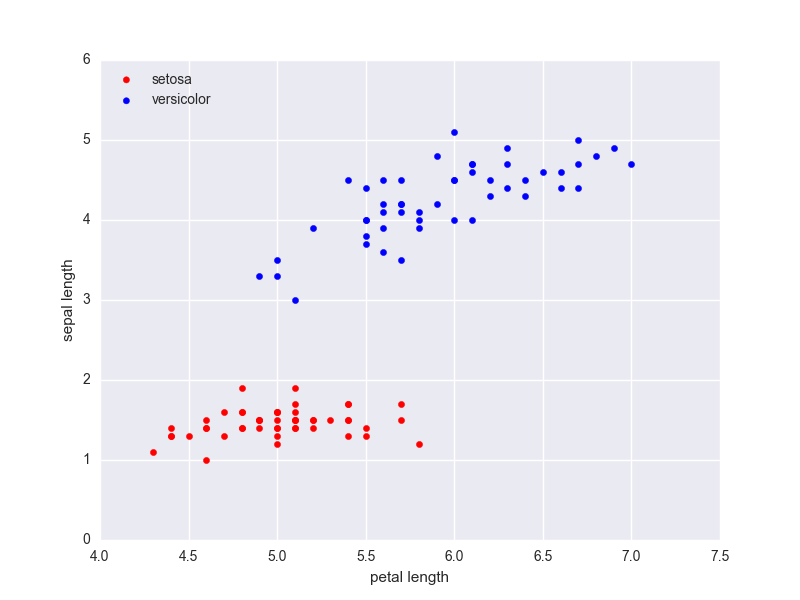
\includegraphics[width=1\textwidth]{fig/raw.png} % Include the image placeholder.png
\caption{训练数据}
\end{center}
\end{figure}

\begin{figure}[H]
\begin{center}
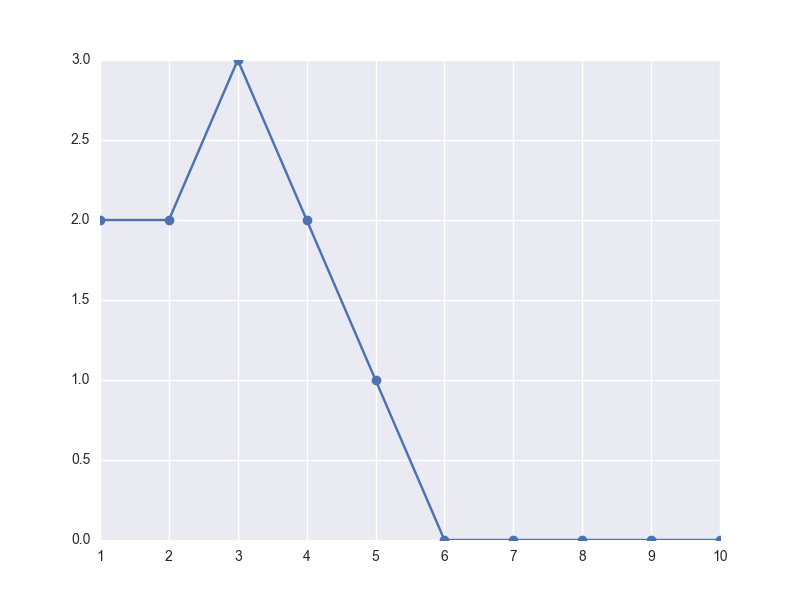
\includegraphics[width=1\textwidth]{fig/errors.png} % Include the image placeholder.png
\caption{每次迭代被错分的数目}
\end{center}
\end{figure}


\begin{figure}[H]
\begin{center}
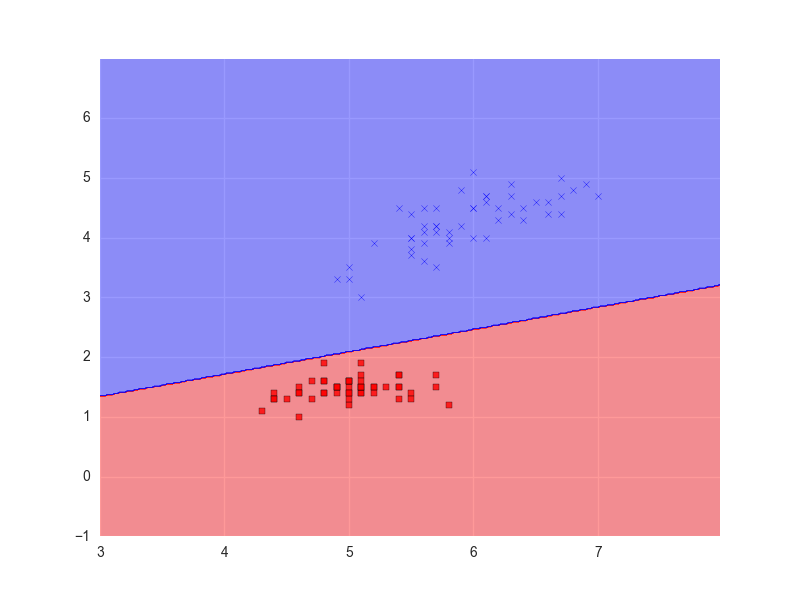
\includegraphics[width=1\textwidth]{fig/decision.png} % Include the image placeholder.png
\caption{Perceptron分类平面}
\end{center}
\end{figure}


%%----------------------------------------------------------------------------------------
%%	SECTION 4
%%----------------------------------------------------------------------------------------
%
%\section{Results and Conclusions}
%
%The atomic weight of magnesium is concluded to be \SI{24}{\gram\per\mol}, as determined by the stoichiometry of its chemical combination with oxygen. This result is in agreement with the accepted value.
%
%\begin{figure}[h]
%\begin{center}
%\includegraphics[width=0.65\textwidth]{placeholder} % Include the image placeholder.png
%\caption{Partial Gradient of $L_\big(\theta \big)$}
%\end{center}
%\end{figure}
%
%%----------------------------------------------------------------------------------------
%%	SECTION 5
%%----------------------------------------------------------------------------------------
%
%\section{Discussion of Experimental Uncertainty}
%
%The accepted value (periodic table) is \SI{24.3}{\gram\per\mole} \cite{Smith:2012qr}. The percentage discrepancy between the accepted value and the result obtained here is 1.3\%. Because only a single measurement was made, it is not possible to calculate an estimated standard deviation.
%
%The most obvious source of experimental uncertainty is the limited precision of the balance. Other potential sources of experimental uncertainty are: the reaction might not be complete; if not enough time was allowed for total oxidation, less than complete oxidation of the magnesium might have, in part, reacted with nitrogen in the air (incorrect reaction); the magnesium oxide might have absorbed water from the air, and thus weigh ``too much." Because the result obtained is close to the accepted value it is possible that some of these experimental uncertainties have fortuitously cancelled one another.
%
%%----------------------------------------------------------------------------------------
%%	SECTION 6
%%----------------------------------------------------------------------------------------
%
%\section{Answers to Definitions}
%
%\begin{enumerate}
%\begin{item}
%The \emph{atomic weight of an element} is the relative weight of one of its atoms compared to C-12 with a weight of 12.0000000$\ldots$, hydrogen with a weight of 1.008, to oxygen with a weight of 16.00. Atomic weight is also the average weight of all the atoms of that element as they occur in nature.
%\end{item}
%\begin{item}
%The \emph{units of atomic weight} are two-fold, with an identical numerical value. They are g/mole of atoms (or just g/mol) or amu/atom.
%\end{item}
%\begin{item}
%\emph{Percentage discrepancy} between an accepted (literature) value and an experimental value is
%\begin{equation*}
%\frac{\mathrm{experimental\;result} - \mathrm{accepted\;result}}{\mathrm{accepted\;result}}
%\end{equation*}
%\end{item}
%\end{enumerate}

%----------------------------------------------------------------------------------------
%	BIBLIOGRAPHY
%----------------------------------------------------------------------------------------
%
% 注意一定要在文中引用才不会出错(至少引用一个)
\bibliographystyle{plain}
\bibliography{bib//perceptron}

%----------------------------------------------------------------------------------------


\end{document}